\documentclass{article}
\usepackage{graphicx} % Required for inserting images
\usepackage[margin=1in]{geometry}   % Marges

\title{6.175 Final Project}
\author{Lasya Balachandran, Sanjay Seshan\\lasyab@mit.edu, seshan@mit.edu}
\date{\today}

\begin{document}

% An approximately one-page description of your project idea is due on Friday 14th.
% Your report should describe the architecture techniques you will explore, design, and implement.
% Typically, most groups should probably first connect the process they wrote to a cache, and then
% upgrade the processor in two dimensions: to go superscalar, or SMT, or multicore, vectors or
% connecting an accelerator to the processor (the lecture about the last two will be given next week).
% 1
% You might also want to use an FPGA for your project, if you want to do so, you should say it in
% your proposal.
% For projects that would not be directly related to processors, you will need to be already very
% familiar with the domain and specific application you are trying to tackle and you should send us
% an email to fix a meeting with us next week to decide on reachable objectives.


\maketitle

\section{Multi-core Processor}
Our first plan is to implement a multi-core processor. To do this, we will build off of our Processor and Cache labs and implement a shared cache hierarchy that maps to a main memory unit.\\ 

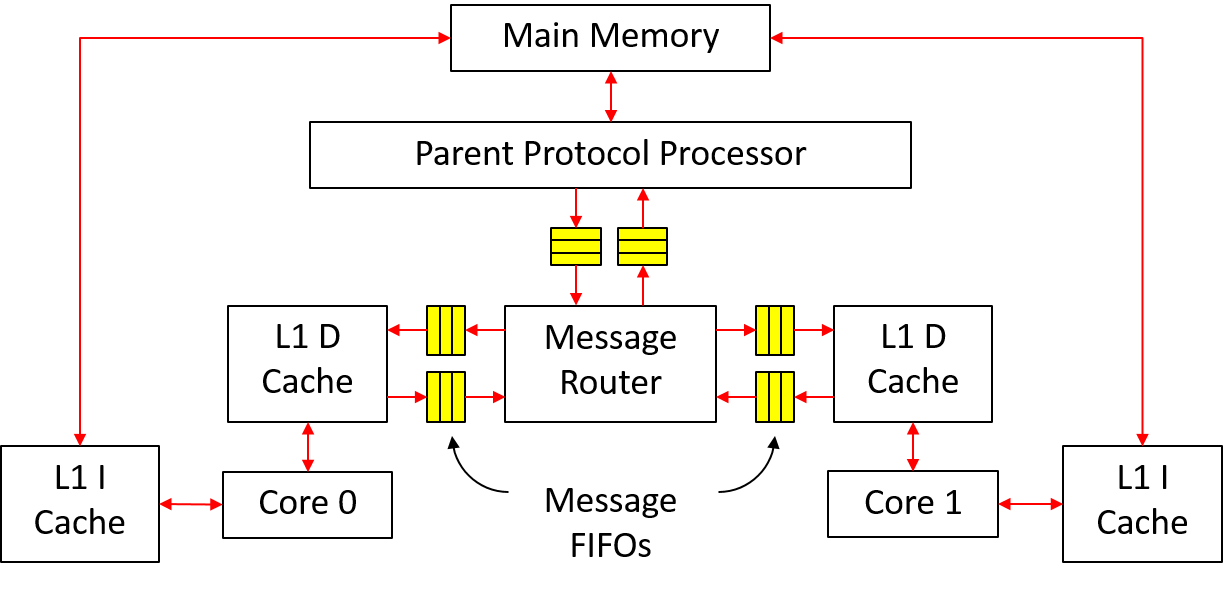
\includegraphics[width=10cm]{system.png}\\

We will include two cores, so the processor will be able to run two instructions at the same time. 
% We will also include a series of RISC-V cores for each thread/each program. 
These cores communicate using a message router to enqueue memory requests. Each core shares a single memory for instruction and data accesses so we will work to develop a hierarchy that will allow shared data usage. This means that higher cache levels will have to force an upgrade on the cache when shared core memory is used to avoid overwrites. Each core should be modular and easily scaled to meet the requirements of the system.

We will have our system consist of a variety of parts. 

The first is the message FIFO. This is used to transfer upgrade and downgrade responses in a cache hierarchy. This works by having a response FIFO and a request FIFO that together form the message FIFO with associated logic. 

We then have a message router to connect all the cores' L1 caches to the parent protocol processor. This part will send messages from the parent to the right L1 cache and vice versa. 

Next, we will have a L1 data cache for each core. This is generally a normal cache interface.

Finally, we have the parent protocol processor which will handle all the messages to and fro memory and the cache. It handles upgrade and downgrade requests. 

% Multi-core processor and run on FPGA
\section{FPGA}
Furthermore we plan to run this system on an FPGA unit. This unit will be cloud based and provided by the 6.175 instructors. Since the multi-core processor will likely only run on the server-based unit rather than the small FPGA, we will use the server-based one. We expect that this will involve some work with Verilog and learning to program the controllers. The Bluespec compiler will generate the Verilog code, from which we will use the associated synthesizing tools to push to the FPGA. 

\section{Other}

We expect that we will have to first merge our code from the Processor and Cache labs to create a fully functioning pipelined processor. We will also add register and memory access bypassing. We will also have to modify these afterward to implement the aforementioned properties. This will still be implemented in a four stage pipelined processor.

\section{Evaluation}

We propose a series of tests to evaluate our system.
\begin{itemize}
    \item Run two different programs, such as two different sorts, on each core
    \item Run two different sets of instructions
    \item Distributed matrix multiply that will divide operations between each core
\end{itemize}

We will use the timing results on this and a standard single core processor to evaluate the improvement in performance. 

\section{Sources}

http://csg.csail.mit.edu/6.175/labs/project-part2.html
\\
Course material from Canvas

\section{Weekly Updates}
\subsection{Week 0}
Initial version of the outline above.
\subsection{Week 1}
We have outlined above in more detail our plans to implement our system in the coming weeks. Next week we will start on the actual code for the Multi-core processor. Eventually we will start learning about FPGAs.
\subsection{Week 2}
Worked to create a L1 and L2 cache within a single core processor. Worked to merge the cache code with the RISC-V processor code. We created a two layer cache with 32-bit addressing.

\end{document}
